\documentclass[12pt,a4paper,table]{report}

\usepackage[utf8]{inputenc}
\usepackage{amsfonts}
\usepackage{amssymb}
\usepackage{setspace} 
\usepackage{graphicx}
\usepackage{array}
\usepackage{pdfpages}
\usepackage{mathtools}
\usepackage{hyperref}
\usepackage{nameref}
\usepackage{tabularx}
\usepackage[]{subcaption}
\usepackage[stable]{footmisc}
\usepackage{float}
\usepackage{bookmark}
%\usepackage[table]{xcolor}

%this is to make the \ref and \label command work at any text
\makeatletter
\let\orgdescriptionlabel\descriptionlabel
\renewcommand*{\descriptionlabel}[1]{%
  \let\orglabel\label
 \let\label\@gobble
 \phantomsection
  \edef\@currentlabel{#1}%
 \edef\@currentlabelname{#1}%
 \let\label\orglabel
  \orgdescriptionlabel{#1}%
}
\makeatother



\title{Valens - An Android application system to detect fall risk among the elderly \\Group 8}
\author{
  Vassdal, Johannes Willumsen\\
  \texttt{johannes.vassdal@gmail.com}
  \and
  Aamot, Elias\\
  \texttt{eliasaa@stud.ntnu.no}
  \and
  Tomren, Filip Andre Larsen\\
  \texttt{filip@tomren.it}
    \and
  Pham, Dat-Danny\\
  \texttt{datdanny@hotmail.com}
    \and
  K\"{u}c\"{u}kyareli,Tayfun\\
  \texttt{tayfun.kucukyareli@live.de}
}

\begin{document}
\onehalfspacing
\maketitle
\tableofcontents

\chapter{Introduction}

Damage from falling is the main cause for hospitalization among the elderly. In addition to the enormous costs incurred to society, falling is also a cause of great personal tragedy. As the use of computational devices becomes more common, it seems natural to examine how such devices can contribute to preventing fall-related accidents.

This project is a cooperation between SINTEF and a group of students at NTNU, as a part of the European research project FARSEEING. The students participate as a part of the course IT2901 - Informatics Project II.

The general goal of the project is to explore potential uses for smart phones in fall risk assessment and prevention. Specifically, the goal was to develop a model for fall risk level based on movement detected by common sensors found in Android smart phones, and build an API to make the model accessible for third-party developers.



\section{IT2901}
IT2901 - Informatics Project II is a course given at NTNU, where a group of students are given a project to work on independently over the course of a semester. The projects are provided by private and public enterprises in cooperation with NTNU. The university provides a supervisor to give the students feedback throughout the semester, but the students themselves are responsible for direct communication with the customer. The course is worth 15 ECTS, which amounts to approximately 20 hours of work per week for each student. 

\section{Group introduction}
The group consists of 5 members, four of which were from Norwegian University of Science and Technology, and the remaining student was an exchange student from Germany, Technical University of Dortmund. The members had experience with programming and project development with the programming languages Java and C, but no experience with any Android application development. 

\section{Stakeholder introduction}
In addition to the developers, the following parties were stakeholders in the project.

\subsection{SINTEF - Customer}
The customer was ``Selskapet for INdustriell og TEknisk Forskning ved norges tekniske hoegskole", or SINTEF for short. The person representing SINTEF was Babak A. Farshchian, Adjunct Associate Professor at NTNU.

\subsubsection{FARSEEING}
``FARSEEING is a collaborative European Commission funded research project with 11 partners distributed in 7 EU countries. It aims to provide a thematic network focusing on the issue of promoting healthy, independent living for older adults. FARSEEING aims to promote better prediction and prevention of falls and to support older adults with a focus on ICT devices and the unique proactive opportunities they can provide to older adults to support them in their own environment''.\footnote{Quote from the "About Us" section of the FARSEEING website \url{http://farseeingresearch.eu}}

\subsection{Target audience}
The target audience for the system are:
\begin{itemize}
\item Elderly that are self-sufficient and relatively healthy, but have some concerns regarding their own stability. They benefit from the application as it provides feedback about their risk level.
\item Health personnel. The application can work as an indicator for fall risk among the patients, and perhaps provide insights into possible 
solutions and causes to the falling problem.
\item Concerned relatives.
\end{itemize}

One major problem that was pointed out by the health experts is that the first target audience does not, in fact, exist. Falling is an enormous taboo, and even people with a history of falling tend to convince themselves that every fall is an individual exception. To cope with this, the application has to be marketed as a general health promoter when targeting the elderly, but run fall risk detection in the background. Targeting the other two audience  groups, the application can still be marketed as originally planned. 

\section{Interested parties}
Groups who are not stakeholders, but still have been of great help.
\subsection{Medical Experts}
Profs Jorun L. Helbostad and Beatrix Vereijken provided invaluable help with understanding questions from the medical domain. They were also associated with the FARSEEING project.
 \subsection{Supervisor - Tinna T\'{o}masd\'{o}ttir}
The developers were assigned a supervisor from the institute. The supervisor, Tinna T\'{o}masd\'{o}ttir, gave guidelines and feedback on how to build the reports and make documentation. She took part in evaluating the project.

\chapter{Requirements}
The requirements for the different parts of the project were about the requirements for the application, the underlying model and content provider, and the documentation for the model and content provider. 

\section{Final requirements}
Several meetings with the customer and health experts led the initial requirements to be out of date and a little vague which led to new and updated requirements.

\subsection{Functional requirements}
\begin{itemize}
\item An Android content provider that stores and makes the data available for other applications through an API. The content provider shall has the ability to show requested data apropiatly without any loss of information and in the way how the user wishes
\begin{itemize}
\item Measure gait speed: The application shall be able to detect the speed of the users gait so that this information can used as a element in the whole detection process. Thus the costumer required in order to detect the main parameter for falling.
\item Measure gait variability: The application shall be able to detect the variability of the users gait. That will be one of the main part for understanding its fall behaviour and the reasons of his falling down. Thus the costumer required in order to detect the main parameter for falling.
\item Measure steps: The ability to counting the steps in order to use their amount as a parameter for the walk/fall statistic.
\item Filter out noise in terms of bad and unnatural movements.
\end{itemize}
\item An example application that can visualize this data and represent them in a pedagogical manner.
\begin{itemize}
\item Ability to do self-tests: This functionality shall give a feedback for the user. Thus the costumer required in order to include the user in the health process.
\begin{itemize}
\item Reaction speed: This application shall give the time of the users reaction to include it in the detection.
\item Stand up sit down capability
\item Balance tests: This part of the application is to understand the balance of the user to include it in the detection.
\end{itemize}
\end{itemize}
\item Documentation on the content provider that can be referred to
\end{itemize}	

\subsection{Nonfunctional requirements}
\begin{itemize}
\item 80\% of the elderly should manage to use the app within 10 minutes of education given that they have some prior knowledge of smartphones.
\item Midly visually impaired should be able to use the application.
\item Color blind should be able to use the application. These shall fulfilled for the reason that the application shall fulfiill the requirement of easy-usability.
\end{itemize}	


\section{Understanding the requirements}

The requirements were specified after several meetings with the customer. The understanding the group had of the requirements before meeting the customer was not sufficient to create a set of requirements. The requirements were also subject to change as the project progressed. \\

The meetings served their purpose, and filled in a lot of holes that were missing from the preliminary description:
\begin{itemize}
\item The development process in question \footnote{See Chapter \ref{def:devProcess} for a description of the development process} uses a iterative approach. This essentially means that the requirements expands as the time goes, and to define the requirements from the beginning is impossible. This decision was made in collaboration with the customer.
\item The team at SINTEF got a wide range of experts to help the group with health-specific features, e.g. making the algorithms to recognize movements.
\item The customer expected weekly meetings with the whole group present, and that goals had been achieved before each meeting. At each meeting a new goal was set.
\end{itemize}

\section{Initial requirements}

According to the project description, the following should be developed:
\begin{itemize}
\item A model of physical movements based on common movement sensors found in Android smart phones.
\item An Android content provider that stores and makes available the data in this model through an Application Programming Interface(API).
\item An example application that can visualize this data. Thus for making the result visible and transparent.
\end{itemize}
\section{License}
The results of the project was intended to be released under the Apache 2.0 license. It is an open source license, which can be found  at the following web site: \url{http://www.apache.org/licenses/LICENSE-2.0.html}\\
Highlights of what can, cannot and must be done under the license is described here:\\
\textbf{Must be done}
\begin{itemize}
\item include copyright
\item include the license
\item state what changes has been made
\end{itemize}
\textbf{What can be done}
\begin{itemize}
\item use copies of the licensed work without paying
\item use the content with commercial products later
\item modify the licensed work as desired
\item the work can be distributed as desired
\end{itemize}
\textbf{Cannot do}
\begin{itemize}
\item trademark the licensed work
\end{itemize}
The specific terms can be found at the mentioned address, and has also been included in the appendix, see \ref{appendix:license}, along with License and Notice files.

\section{Testing}
The tests were done by the black-box principle of testing, meaning that all the tests consider is, with no attention given to the inner workings of the methods. Because of the team following an agile development method, it was possible to create and test test-cases in short order. The test-cases were therefore written with results included.
The tests are corresponding screens for the tests were as follows:
\begin{description}
\item[Name Entry] is associated with tests 1.x, both when program is started the first time, and when name-change is initiated from settings.
\item[Event Details Screen] is associated with tests 2.x.
\item[Statistics Screen] is associated with tests 3.x.
\item[Clear history] can be initiated from settings screen and is associated with tests 4.x.
\item[Related people Screen] is associated with tests 5.x. 
\end{description}

\begin{figure}[h]
\label{tab:testList}
\caption{List of tests for the application}
\begin{tabular}{|p{\textwidth /4}||p{\textwidth /4}|p{\textwidth /4}|p{\textwidth /4}|}
\hline
Test number & Input value& Actual Result& Expected Result \\
\hline
\hline 
1.1 & Any valid name & Hello: + name & Hello: + name \\ 
\hline 
1.2 & Empty name-box & Hello: &Hello:  \\ 
\hline 
2.1 & Remove event button clicked & Event removed & Event removed \\ 
\hline 
2.2 & Keep event button clicked & Event is kept & Event is kept \\ 
\hline 
3.1 & Timeslot set to 10 min or less & Data from correct timeslot displayed & Data from correct timeslot displayed \\ 
%\hline 
%3.2 & • & • & • \\ 
\hline 
4.1 & Clear History Button Clicked & History Cleared & History Cleared \\ 
\hline 
5.1 & Add existing contact button clicked & Contact shows up on appropriate screen  & Contact shows up on appropriate screen \\ 
\hline 
5.2 & Create New Contact function used & New Contact shows up on appropriate screen & New Contact shows up on appropriate screen \\ 
\hline 

\end{tabular} 
\end{figure}

\chapter{Prestudies and Alternate Solutions}
During the planning stage, the group was able to identify two areas which required research:
\begin{description}
\item[Domain knowledge:] No member of the group had any familiarity with the application domain, neither with the specific domain (fall studies) nor any of the related domains (like healthcare, medicine or sport science). A basic understanding of the domain is critical for communication with the expert group, as well as for the ability to develop and assess solutions independently of the expert group.
\item[Related software:] Related applications function as sources of inspiration, proofs of what is feasible to implement or even as aids during programming. Open source software can be partially or entirely incorporated into the code. Knowledge of related software can thus increase development efficiency.  
\end{description}
For each of the two areas of research, one member of the group was assigned to research and compile a concise report, so that the rest of the group could efficiently attain the required knowledge.   

The two reports are reproduced in the following sections.

\section{Falling: Causes, Consequences and how to avoid it}
This report collected information from several sources on the subject of falls among the elderly. Particular focus is given to risks and avoidance strategies.

\subsection{Risk factors}
There are several factors that predicate risk of falling. Typical risk factors are:
\begin{itemize}
\item 
\textbf{Biological risk factors (sorted by order of significance):  \cite{fallsRubenstein}}
\begin{itemize}
\item Muscle weakness
\item Balance deficit
\item Gait deficit
\item Visual deficit
\item Mobility limitation
\item Cognitive impairment
\item Impaired functional status
\item Postural hypertension
\end{itemize}
\item 
\textbf{Behavioral risk factors(Not in sorted order):}
\begin{itemize}
\item Inactivity \cite{cdcComProg}
\item Medications \cite{cdcComProg}
\item Alcohol use \cite{cdcComProg}
\item Living alone \cite{housing}
\end{itemize}
\item 
\textbf{Home/environmental risk factors(not in sorted order): \cite{WHO}}
\begin{itemize}
\item Bad footwear or clothing.
\item Dangers in the house or in public places.
\item Unfamiliarity with walking aids such as canes, crutches, walking chairs.
\end{itemize}
\end{itemize}

A fall is normally caused by the interaction of two or more of these risk factors, but home or environmental risk factors cause only 30-50\% of all falls\cite{fallsRubenstein, cdcComProg}. What this means is that more than half of all falls happen without any influence of environmental factors. Also, in most of these cases where external factors play a role, the fall is in reality caused by an interaction between these and physiological aspects. The second and third most common single causes of falling are gait/balance disorders and dizziness/vertigo, followed by \emph{drop attacks}, which are sudden falls without loss of consciousness or dizziness\cite{fallsRubenstein}. As the project task is to develop a model for physical movement, it might be necessary to down-prioritize identifying risk for dizziness/vertigo and drop attacks, as well as ignore external factors, in order to focus purely on physiological aspects, such as gait or balance.

Many older adults are unaware of their risk factors, and therefore unable to take preventive actions. Even older adults with a history of falling have normally been given little education about the potential risk factors. Any sort of risk assessment, is therefore be very beneficial, especially when the results are discussed with a healthcare provider\cite{cdcComProg}. This fact illustrates the usefulness of the planned application. 

It has been shown that many of the biological risk factors can be reduced effectively by preforming regular physical activities. Specifically strength, gait and balance has been shown to be improvable by simple exercise regimes - even for frail patients - in a number of studies\cite{LMTassessPrev, cdcComProg, WHO}. A potential focus area for the app can therefore be encouraging exercise and healthy lifestyles.

\subsection{Advice for prevention}
The individual can easily reduce the risk of falling greatly by taking certain measures. A list of measures normally, by the authorities, recommended for older people in the target group is given below\cite{cdcYouPrevent}:

\begin{itemize}
\item Begin a regular exercise program.
\begin{itemize}
\item Exercises that improve balance and coordination are the most helpful.
\item Is the only measure that by itself reduces the risk of falling independently of individual circumstances. 
\end{itemize}
\item Have your health care provider review your medicines, even over-the-counter ones.
\begin{itemize}
\item Avoid medicines that can make you dizzy or sleepy.
\end{itemize}
\item Have your vision checked.
\item Make your home safer.
\begin{itemize}
\item Remove or fasten small rugs and carpets.
\item Remove wires and cords away from commonly taken paths. Tape wires to the walls, and if necessary install an additional power outlet.
\item Keep items where you can reach them without having to climb. If you have to use a step stool, get a stable one with handrails.
\item Remove loose items that can make you trip (books, papers, clothes, etc.) from the floor and stairs.
\item Add grab bars and non-slip mats to the bathroom.
\item Make your home brighter.
\item Repair broken or uneven steps and handrails in the staircase.
\item Avoid using the staircase more than necessary, for instance by installing a light switch at the top as well as the bottom of the stairs. 
\item Wear shoes, even inside. Avoid walking barefoot or wearing slippers.
\end{itemize}
\end{itemize}

\subsection{Physiological aspects}

The list below explains the physiological factors that contribute to stability. “A marked deficit in any one of these factors may be sufficient to increase the risk of falling; however, a combination of mild or moderate impairments in multiple physiological domains also may increase the risk of falling. By directly assessing an individual's physiological abilities, intervention strategies can be implemented to target areas of deficit.” \cite{LMTassessPrev}

\begin{itemize}
\item Reaction time
\begin{itemize}
\item Hand
\item Foot
\end{itemize}
\item Vision
\begin{itemize}
\item Contrast sensitivity
\item Visual acuity
\end{itemize}
\item Vestibular function
\begin{itemize}
\item Visual field dependence
\end{itemize}
\item 
Peripheral sensation
\begin{itemize}
\item Tactile sensitivity
\item Vibration sense
\item Proprioception
\end{itemize}
\item Muscle force
\begin{itemize}
\item Knee flexion
\item Knee extension
\item Ankle dorsiflection
\end{itemize}
\end{itemize}


There exists an array of tests that can measure the performance on these aspects. Lord et al. \cite{LMTassessPrev} provides one possible set of tests. Some of these are possible to implement in an app, but none of them are based on hip movement.

The test developed by Lord et al. \cite{LMTassessPrev} was used to classify older adults into fallers or non-fallers, and has an accuracy of $75-80\%$ in different experiments. If a test which disregards hip movement patterns performs well, there may be reasons to believe that hip movement is only a minor factor in detecting fall risk. However, 

Walking behaviour seems to be generally associated with falling. Lord et al. \cite{LLKgaitPatterns} shows that there is a negative correlation between falling and steps per minute, stride length and stride velocity. A positive correlation was shown between falling and stance duration and stance percentage. However, these physiological traits are all associated with old age, and old age is associated with falling, so the relation might be quite indirect. On the other hand, stride and stance as physiological aspects that can be measured with relative ease using a mobile phone.

\section{Related Applications}
There exist several other open source programs and commercial programs that solve related problems. These could function as inspiration for design, interfaces and functions, and open source programs can be imported and incorporated into the project. The most relevant related applications will be presented below.

\subsection{Endomondo Sports Tracker}
This is a popular app for exercising. It can be used to track routes, times and progress in training and activities. It uses GPS (and accelerometer) to find position on maps and track the location. Very easy to use, and automatically syncs up to endomondo.com. Has an inspiring design and sync-functionality.

The main part of Endomondo is the inspirational part to get people to move; you can compare yourself to others, e.g. friends, and you have a really easy way to see what an exercise is worth in amount of calories and amount of burgers burned by an exercise.

A lot of aspects from this app can be used during design, especially labelling and representation of data.

\subsection{GPS Status}
This application is used to view detailed status about the GPS system on the phone. Has a very advanced interface with lots of numbers to show information, but for a rookie user the data rarely translates into information.

The app succeeds to use the sensors very heavily.

\subsection{Pedometer}\footnote{Application can be found at \url{https://code.google.com/p/pedometer/}}
An open source app that has a GPLv3 license that is compatible with our Apache 2.0 license. The app uses the same sensors that may be useful for the current project. Taking advantage of this could reduce development cost drastically.

The creator's description of how the step detection algorithm works\footnote{Taken from the FAQ at \url{https://github.com/bagilevi/android-pedometer}}: \textit{Basically, it aggregates the sensor values, finds the maximum and minimum, and if the difference is bigger than a value (which depends on the sensitivity setting) then it counts it as a step. There's is some additional optimization, which I arrived to through experimentation.}

\subsection{GPS Tracker}\footnote{Application can be found at: \url{https://code.google.com/p/open-gpstracker}}
This program adds the capability to store and review where you and your Android device have been. Basically you press record at the start of your trip and your phone stores the route you take. This route is drawn real-time on the Maps functionality of Android or in the background with an idle device. The route is stored on your phone for review and further use. The applications tracks location by GPS, hence the name. An accurate description of the program type would be a GPS logger.

It contains the ability to log location, something that might prove useful for current project. Since it is open source and has a compatible license (GNU v3), it can be incorporated easily.

\subsection{Summary of interview with medical professionals}
This is a summary of the information gathered by a meeting with two medical professionals and the customer.
\textbf{Present:} All group members, Babak Farshchian, Jorunn L. Helbostad, Beatrice Vereijken \\
\textbf{Time:} 14.15-15.37\\
\textbf{Place:} St.Olavs Hospital\\
The plan was to have a short presentation, a short GUI demonstration, and then discuss and interview with the interviewees. \\
\subsubsection*{Feedback on Interface and Presentation of the program}
\begin{itemize}
\item Immediate and summarized feedback was desired, as it would be more helpful than feedback later.
\item A focus on falling is not a selling point, try health or lifestyle instead
\item Menu is not obvious to people without android experience
\item Interface seems too complex for target groups
\item Text might be too small
\item Graph needs more contrast 

\end{itemize}

\textbf{Feedback on program functionality}
\begin{itemize}
\item Feedback should be tailored to particular groups
\item Self-testing can be useful for reducing risk and keeping awareness,
\item Small tests to measure reaction time, for example reaction to light or sound
\item Researchers could also be interested in data gathering
\item Measuring transitions between sitting/lying and standing up
\item Compare behavior on a weekly basis will give an overview of whether things are good or not
\end{itemize}

\textbf{Feedback on medicinal stuff}
\begin{itemize}
\item Preventing inactivity over time is useful to reduce risk
\item People with stability problems increase risk when moving much
\item Variable gait pattern is useful for predicting risk
\item Step time is more robust (and hopefully easy to measure)
\item A common exercise is to take a step forwards, sideways, backwards, sideways (measuring a box)
\item People in risk group are those who cut out walking, taking the bus, want help from others around the house
\item Irregularity in speed and length is important to look for
\item Appropriate movement amount for gender and age group is usually known
\item Time needed to turn in place
\end{itemize}

\subsection{Informal usability test}
During the meeting with the medical experts, the group gave an small and informal usability test to the two experts. 

\textbf{Prototype test}\\
\textbf{Subjects: Beatrice \& Jorunn}
\\

\subsubsection{Procedure}
This test was mainly focused on how intuitive it was to navigate the application system and how easy it was to understand the data received by the system. The procedure for this was to give the test subject a phone with program installed. They would then be asked to accomplish a few short tasks, and the observers would rate how easy the subject accomplished the tasks. 

\subsubsection{Results}
The data received from the system was easy to spot and easy to understand. The subjects had some difficulty finding the menu button for the first time, but had no problems with using it later on. It was overall relatively easy to navigate the system. However, the complexity was likely to be a bit much for the target group.

\chapter{Project Management}
\section{Terms}
Here follows a description of terms that are useful to understand how the project management functioned. 

\begin{description}
\item[Scrum] \label{def:scrum}is an popular agile software development methodology. This means that the work is done in increments called sprints, and daily meetings are held to update the rest of the team on progress and problems. The scrum process also has roles for team members, in particular a team member called scrum master who handles contact between the development team and people outside the team.

\item[Sprint] \label{def:sprint} is a period in which work is planned and done. It has a duration of one week. At the end of each sprint the group is updated on progress achieved, and sets goals for the next sprint. 
\item[Kanban-board] \label{def:kanban} is a visual aid that was used to display work packages, with content, people assigned to each package, and status of work package (to do, currently worked on, finished). The intent was to simplify and organize the work being done and work in need of finishing.
\end{description}
\section{Development process}

The customer favored the use of an iterative approach to the development process, where every sprint added a new layer of functionality, either to the application or the underlying model. Each sprint lasted for a period of 1-2 weeks, and the exact content was worked out in collaboration with the customer. Short term plans were favored over longer plans, due to the flexibility provided. While this made formulating definite goals for the final product difficult, the customer and the group were in agreement that due to the research intensive nature of the project, a high degree of flexibility was required. 

It was decided that the developers would have online meetings twice a week and an offline meeting once a week. 
The working hours were set to not less than 20 hours a week, but the developers were free to choose when to work themselves. This number was the expected workload for the course, and made a reasonable target for work per week. The meetings with the team was set to two times per week instead of once per day, so it could fit with the schedules of the team members. This was different from other agile methods like Scrum, but if was a necessary adaptation to fit meetings into the entire teams schedule. Updates were shared among the team members with email, trello\footnote{See \pageref{def:trello} for more info}, and it's learning as a replacement for daily meetings.

\section{Plans}

Nearing the end of every sprint, the customer and group agreed upon the content of the following sprint. This list has been placed in Figure \ref{tab:sprintList}, and provided a short summary of what was accomplished in a particular time-frame. 


\section{Team Roles and Organization}
There was not much place for specific roles among the group, as it was a small group, and the project required that all the members were capable and willing to work at all the tasks. This makes a difference from development models with specific roles and tasks assigned. Roles that were set for the group were therefore mainly organizers, so that one person was to keep awareness of what work needed to be completed in a particular domain, and share it with the rest of the group:

\begin{description}

\item[Group Leader] Elias was made organizer, and got the responsibilities of reminding the group of what to do.
\item[Document-organizer] Johannes was tasked with organizing documentation and distributing the work of writing the report to the group. 
\end{description}

\section{Comparison}
The development model used by the group was a form of agile development. Other well-known examples of agile methodologies were scrum and extreme programming. 

\section{Management Tools}
 
\begin{description}

\item[Trello]  \label{def:trello} was a collaboration tool with the ability to create interactive kanban-boards online. This use of this tool was to allow the group to coordinate tasks that were to be done, and the progress on the tasks, and which members were to work on which task. 
\item[It's learning] was used to distribute information that was not time -critical, with a message board being used. It's learning would not send messages when a new topic or message appeared, so it's use for time-critical messages or making sure that everyone would read it was limited. 
\item[Email] was used for time-critical communication, and for information that needed feedback swiftly, often within the same day.
\item[Github] \label{def:github} was used to share code, and to describe and mark issues found in the code when problems were discovered. The relevant issues could then be discussed on the website
\end{description}
\section{Work Breakdown Structure}
With a development methodology that stresses short term goals, it is only possible to plan WBS for the current period. After the customer has specified the goal for the following week, we immediately sat down and defined the WBS for the given period. This was, a WBS was developed incrementally by adjoining the new WBS to the previous. The WBS was made in graphical form, as can be seen in Figure \ref{fig:WBS}.

\begin{figure}[p]

\setlength\fboxsep{0pt}
\setlength\fboxrule{1pt}\noindent\makebox[\textwidth]{%
 \fbox{
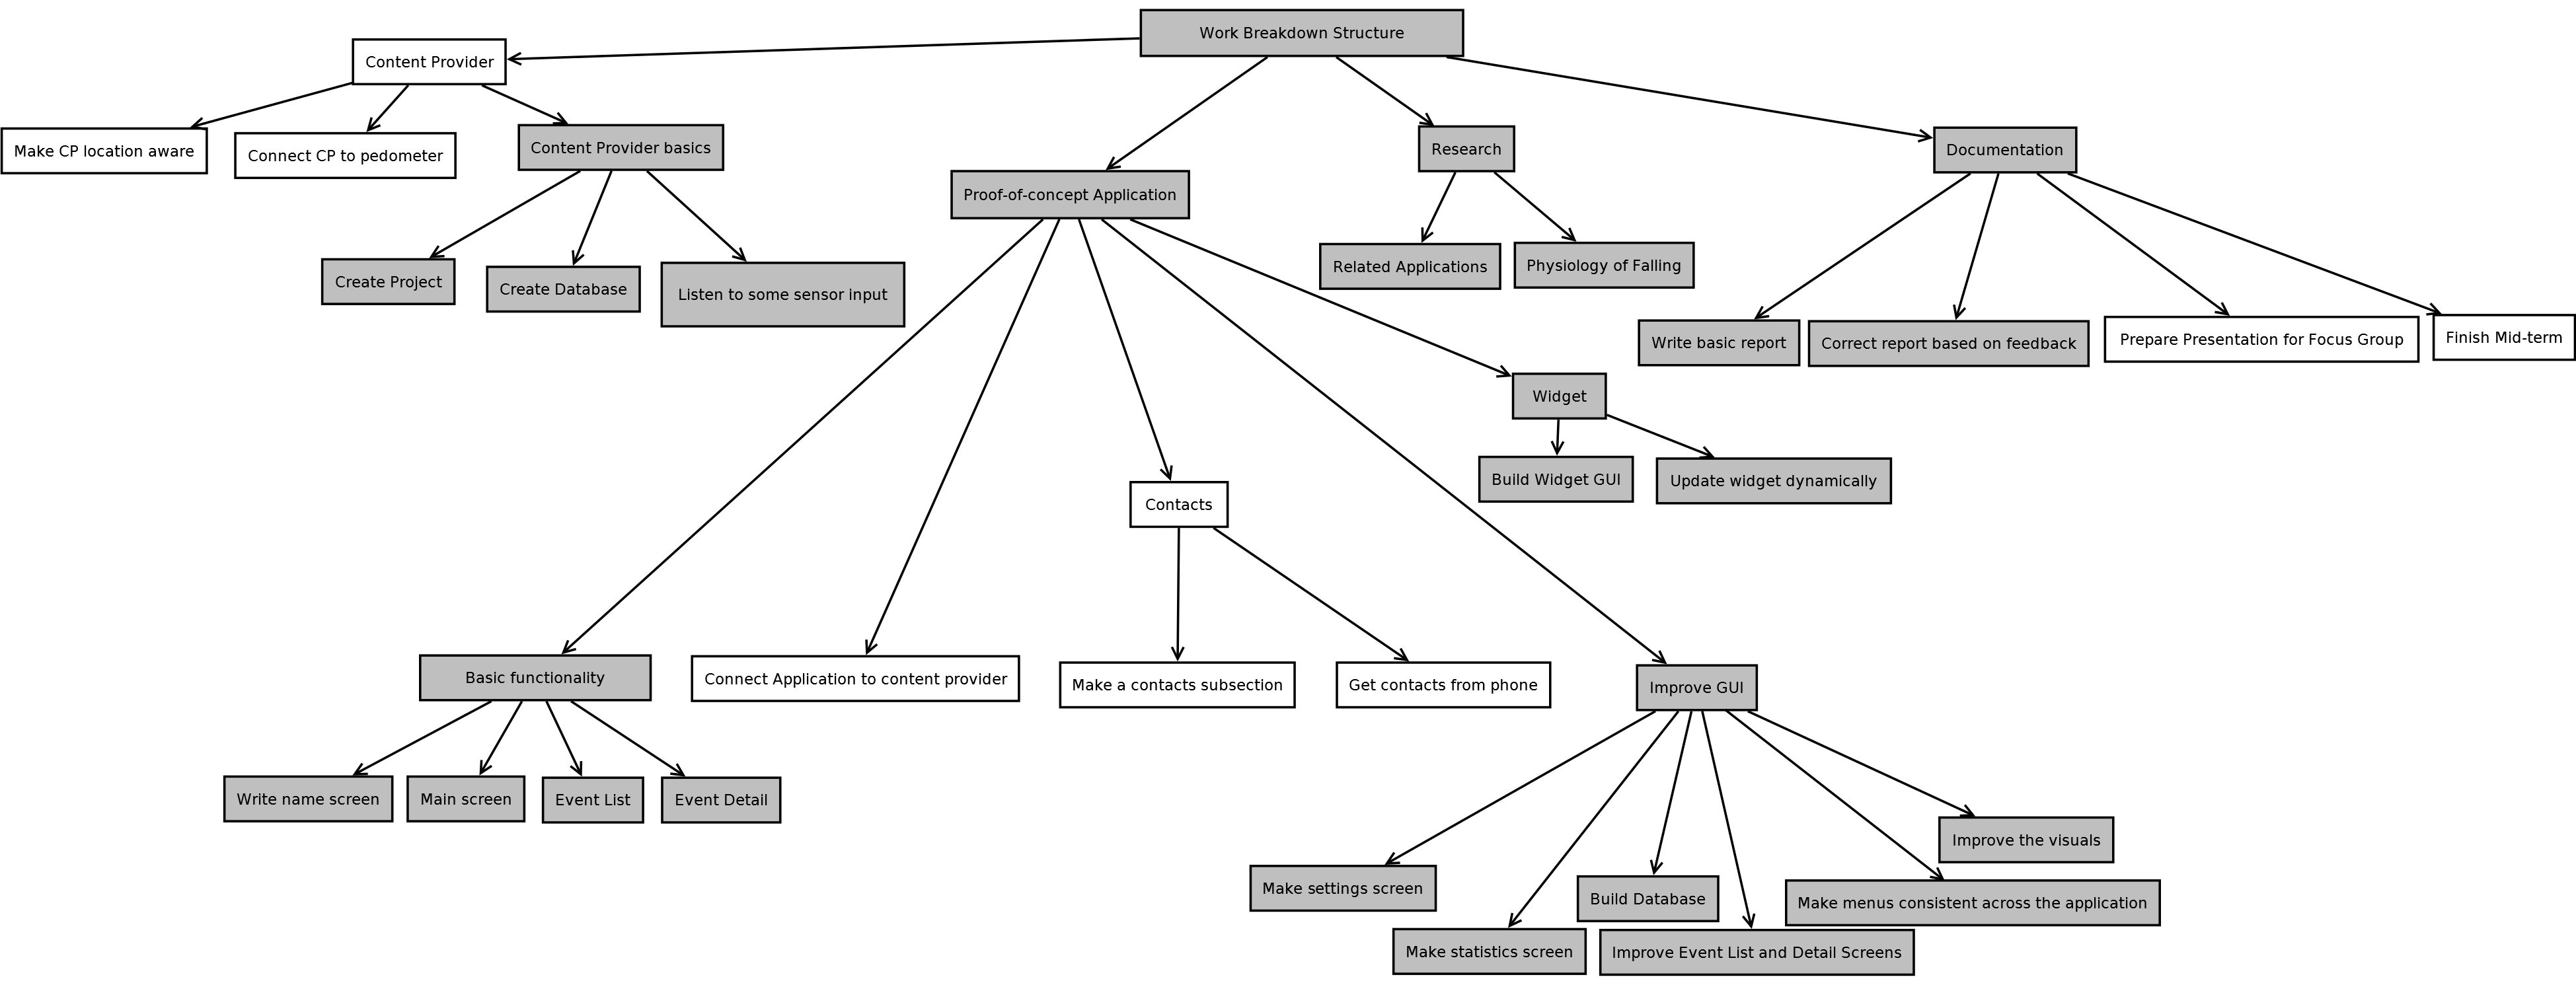
\includegraphics[width=1.45\textwidth , angle=270]{Res/WBS15313.png}
}
}
\label{fig:WBS}
\caption{The current WBS}
\end{figure}
\chapter{Development Environment}

\section{Code-sharing}
It was requested that the group would use the tool Github to share code and perform version control. Github had browser-based interfaces and downloadable clients, meaning all the members of the group could make use of it. \\
The repository that was to be used for the project was called "Fall\_Prevention\_2013". The first content shared in the repository was this report, in form of .tex files and a .pdf. Later this repository would also be used to keep the code in order. 

\section{IDE}
The demands from the IDE was as following:
\begin{itemize}
\item Could be used with Android programming
\item Was sufficiently understood by the team members to be used
\end{itemize}
To fill these requirements, and because there was plenty of tutorials that could be found, the group decided to use the Eclipse IDE, with add-on's to more easily code and deploy towards Android. 

\section{Prototyping}
Graphical prototyping was done with a service called "proto.io".
\chapter{Implementation}


\section{Overall Architecture}
The product has been implement as a system of independent component applications where each component performs a well-defined task. The motivation behind the modular architecture is two-fold: Primarily, it was desirable that the underlying model for movement and fall risk be independent of the proof-of-concept application, in order to facilitate development of possible future applications employing the model. Likewise, it is desirable to enforce independence between the content provider and the sensor model. Secondly, the standards of Android application development state that a Content Provider should in itself solely provide a interface to the data. This implies that the sensor model, as well as any derivation of secondary data, should be performed in components independent of the Content Provider.

The system that has been designed according to these principles therefore consists of five components: The content provider emph{Valens Content Provider}, the proof-of-concept application emph{Valens Health Helper}, the sensor model emph{Valens Step Detector} and a service of deriving secondary data emph{Valens Content Feeder}. Each of these components fulfils a well-defined role in the total application system: The content provider provides an interface to the data model. The sensor model listens to the sensor data, and feeds the content provider with the timestamps of any detected steps. The Content Feeder listens continually to changes to the data in the content provider. When the data changes, it uses the new data to calculate secondary data, such as gait speed and variability. Finally, the proof-of-concept application demonstrates one simple way in which the data provided by the content provider can be used as a part of a health-promoting app.

\begin{figure}[p]

\setlength\fboxsep{0pt}
\setlength\fboxrule{1pt}\noindent\makebox[\textwidth]{%
 \fbox{
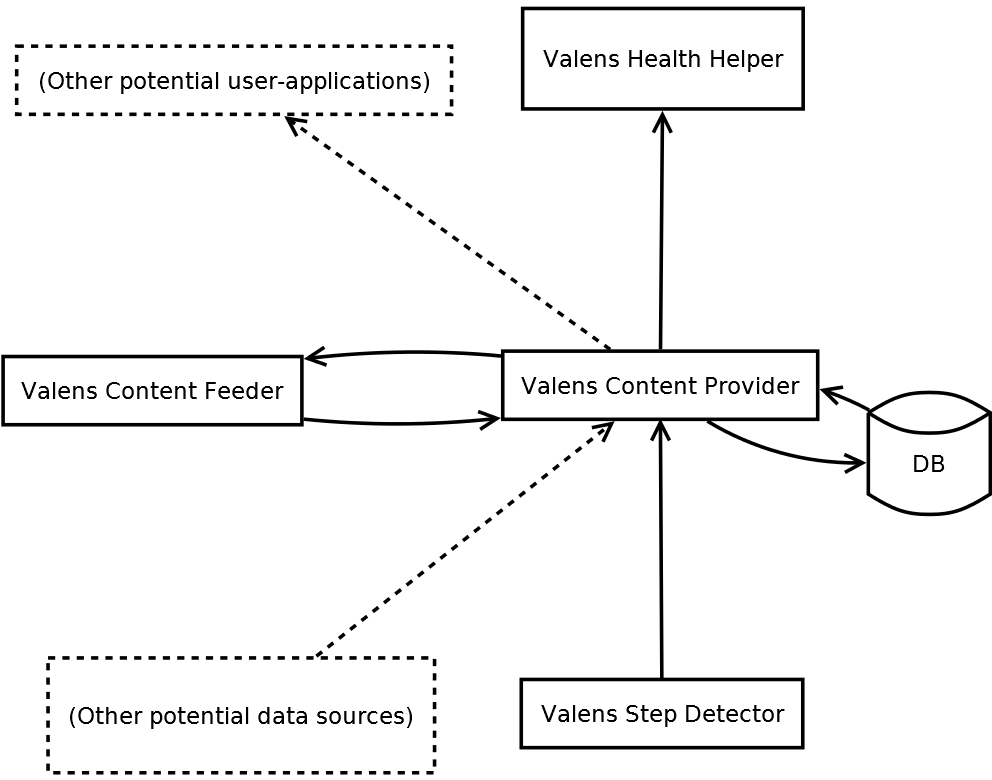
\includegraphics[width=1.45\textwidth , angle=270]{Res/OverallArchitecture}
}
}
\label{fig:Architecture}
\caption{The over-all system architecture}
\end{figure}


\section{Architecture of the App}
The application is made in a way that is common for all android applications. This means that user interface is described in XML layout files that is called in Java code. Strings and resources is placed in a separate folder and file, to be accessed by the code as needed. This is to separate content and layout in the UI. The separation of layout and strings enables different localizations, so that the application can provide a user interface in different languages easily.

As is common in android applications, classes that inherit from the class Activity define a separate screen in the GUI. Because of this, a significant part of all the classes in the application are activity classes. These classes simply define the behaviour of their GUI screen. The flow for the GUI can be seen in Figure \ref{fig:FlowchartGUI}
\begin{figure}
\setlength\fboxsep{0pt}
\setlength\fboxrule{1pt}\noindent\makebox[\textwidth]{
\fbox{
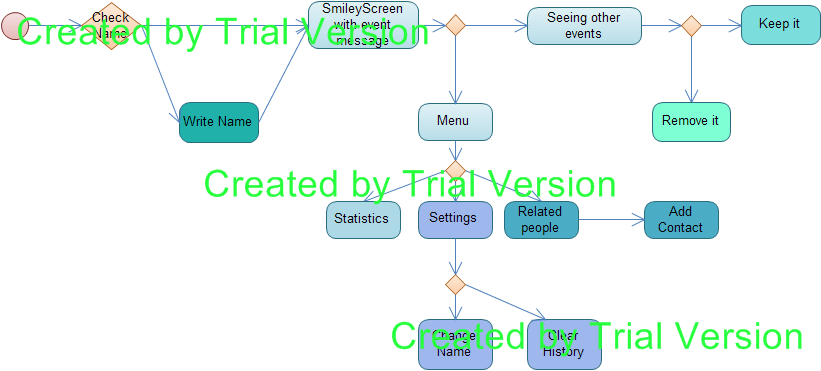
\includegraphics[width=1.2\textwidth, angle = 270]{Res/FlowChartGUI.png}
}
}
\caption{Flow chart describing the Graphical User Interface}
\label{fig:FlowchartGUI}
\end{figure}

Classes that are not activities can be roughly divided into 4 types: Data structure classes, auxiliary classes, connectivity classes, widget classes. Data structure classes simply define a useful data structure in the program. The data structure classes in the app are Event, ContactPerson and RiskStatus. Auxiliary classes help the activities perform their tasks. Most common among these are the adapters that define how elements should be shown in a list view. Connectivity classes are responsible for communicating with the database and content providers. There are two connectivity classes: DatabaseHelper, which does all the work, and DatabaseContract, which specifies the table and column names in the database. While a DatabaseContract might seem redundant, it is common android application practice to use one. Finally, there are the widget classes. WidgetProvider creates the widget and gives it a GUI. WidgetUpdateService is started by the WidgetProvider and takes care of updating the widget when changes happen in the content provider.

\section{Architecture of the Content Provider}
In android, Content Providers provide an interface to structured data of some sort. Access to for instance the list of contacts in the phone, or the phone's calendar is managed through standard content providers. Content Providers provide methods for inserting, updating and deleting relevant data. A major part of the assignment was to implement a Content Provider that gives developers access to structured movement data.

The Content Provider component is conceptually very simple, and consists of four classes:
\begin{description}
\item[CPValensDB]
a subclass of SQLiteOpenHelper, the standard android class for handling database communication. Specifies the procedure for creating the database, as well as upgrading and downgrading the database version. In the current implementation, upgrading and downgrading the database version clears all the data and tables, and creates the database according the details specified in the new database version. In the current version, creating the database consists of creating the tables given in the data model, without feeding any data into the database.
\item[DBSchema]
defines the database model and provides string values for the names of the tables and fields. Employing a database schema to demonstrate the structure of the database is standard in android applications.
\item[ValensDataProvider]
a subclass of ContentProvider, which is the standard android class for implementing content providers. This is the core of the content provider, and describes how queries to the content provider are handled.
\item[Main]
provdides the content provider with a basic GUI.
\end{description}


\section{Class description and diagram}

The class structure of the Applications changed regularly, and the most recent description is in Figure \ref{fig:ClassDiagram}. Older diagrams and descriptions was placed in the appendix. 
\begin{figure}[p]
\label{fig:ClassDiagram}

\setlength\fboxsep{0pt}
\setlength\fboxrule{1pt}
\fbox{
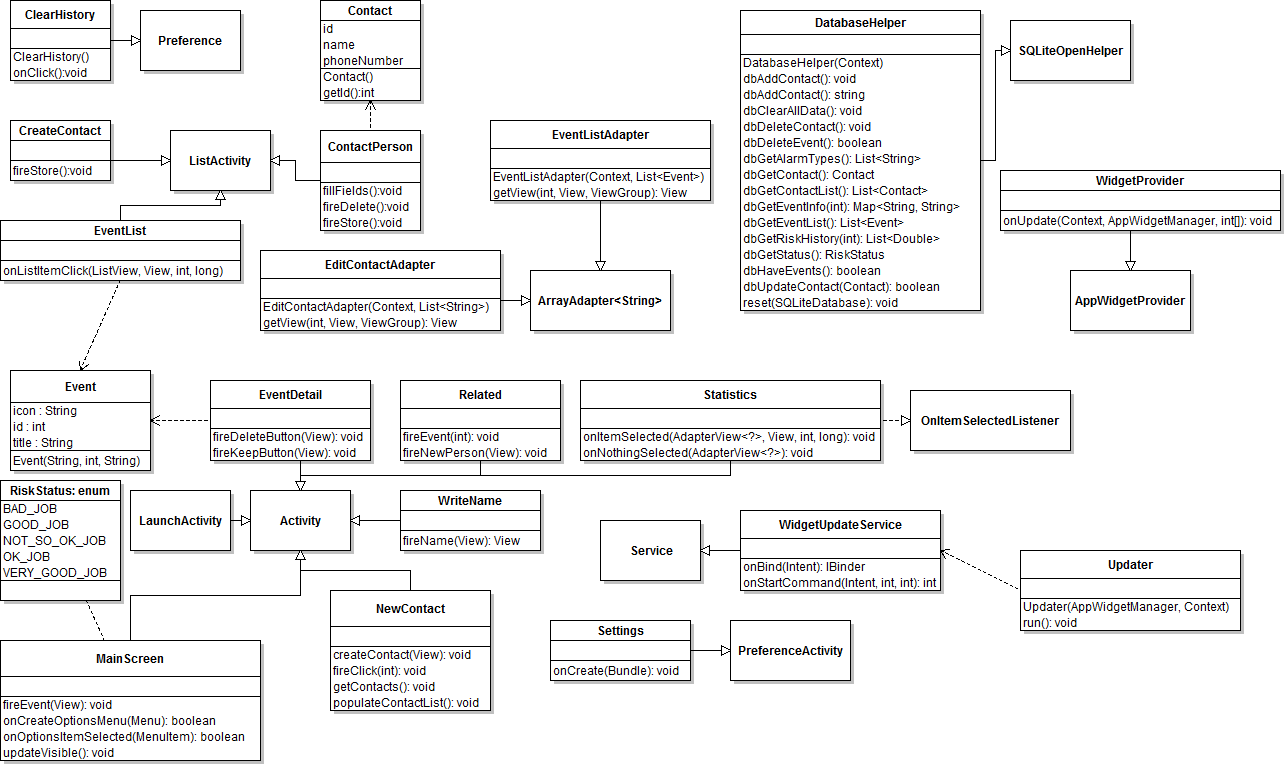
\includegraphics[width=1.2\textwidth, angle = 270]{Res/ClassDiagram}
}
\caption{A class diagram of the current application}
\end{figure}

\section{Architecture of the Valens Step Detector}

Despite being a relatively simple application in terms of lines of code and GUI screens, the architecture of Valens Step Detector has a certain complexity.

\begin{description}

\item[LaunchActivity]
handles the basic GUI for the main screen.

\item[Values]
holds the values of the constants used for step detection.

\item[Methods]
contains most of the functions used for calculation of peaks.

\item[StepMainService]
is main class for the sensor model. Is implemented as an Android Service, and as such, it runs in the continually in the background until the user explicitly stops it. Functions as a SensorListener that listens to input from the accelerometer, and keeps track of the sensor vector lengths along with their timestamp. When enough data has been generated\footnote{Enough data is defined as $m+2k+2n$, where k is the size of the smoothing window, n is the size of the peak strength window, and m is a constant which defines how many time steps one wants to use for step detection. As the first and last $k+n$ steps are not used for step detection (see explanation of the algorithm), only $m$ values will actually be used for step detection.} the StepMainService will launch a DetectStepsThread to detect steps in the given data, before clearing its data\footnote{For reasons that will be explained in the description of the algorithm, $2k+2n$ data points are retained.} to ensure that the maximum memory required by the service remains constant. 

\item[DetectStepsThread]
searches asynchronously for steps in the data provided to it. Step detection is performed in a separate thread so that sensor input is not interrupted by the calculation.

\item[Calibration Classes]
are a group of classes that are used for calibration, that is adjusting the mean and standard deviation to the step patterns of the user. There is one GUI class, one class used for timing and and one sensor class:
\begin{description}
\item[CalibrationActivity]
handles the GUI functions for the calibration screen. When the "calibrate"-button is pressed, it starts a timer that starts the CalibrationStartTask after a certain amount of time has passed, so that the user has time to lock the screen and put the phone in his/her pocket.
\item[CalibrationStartTask]
is a TimerTask that simply plays a sound to indicate that calibration commences, and immediately starts an CalibrationThread. This class only exists because Java requires a TimerTask for the Timer to work properly, and CalibrationActivity can't inherit from TimerTask as it already inherits from Activity and Java does not support multiple inheritance. 
\item[CalibrationThread]
handles sensor input during calibration. When the calibration time has ended, it stops receiving input, calculates $\mu$ and $\sigma$, and terminates.
\end{description}
 
\end{description}


\section{Step Detection Algorithm}
The algorithm used to detect steps is described in this section. The terms not obvious are also described here:
\begin{description}
\item[Gait Speed] is the interval between two steps, and measuring it is useful, as it can be used to measure Risk for falling and as a shorthand for physical ability.
\item[Gait variability] is the standard deviation for gait speed over time. This is significant, because a large variability is correlated with increased risk for falling.
\end{description}
\subsection{Development and purpose of Algorithm}
As the group had little experience in sensor use and signal processing, a series of experiments were conducted to better understand which sensors provide useful information for step detection, and which patterns predicate steps. To this end, a simple app was developed to observe sensor input and store the raw data as a file, which then could be transferred to a computer. A set of Python scripts were written to plot  the data time series. Using Python, the group experimented with different step detection algorithms, and a prototype was developed. Finally, the algorithm was implemented in the Valens Step Detector app, modified to work with live data.

\subsection{Core Algorithm}\label{def:coreAlgorithm}
The current section will explain the algorithm used for step detection, formulated as an off-line algorithm. The following section will explain what changes were made to make the algorithm work for live data streams.

Experiments showed that the accelerometer consistently gave the most predicative feedback patterns for step detection\footnote{None of the android phones available to the group at the time had a working gyroscope. It is suspected that a gyroscope can replace or supplement the accelerometer for more precise step detection, but this should be tested empirically.}. Furthermore, it was found that the total acceleration was a better predicator of steps than acceleration along any of the single axes individually. To exploit this, a pre-processing step calculates the vector length in euclidean space of the raw acceleration vector.

Detecting steps based on a time series of acceleration vector lengths reduces to peak detection in the time series graph. The step detection algorithm is therefore essentially a generic algorithm for peak detection in noisy data. The noise in the data originates from noise in the sensor readings. To cope with the noise, the data is first smoothed using a moving average\footnote{That is, every data point has its value set to the average of itself and the k neighbors before and after it, where k is a constant referred to as the \emph{window size} of the smoothing.}. A larger value of k gives a smoother curve, but a too large value of k may flatten the graph too much.

Subsequently the program runs the main peak detection algorithm, which consists of the following steps:
\begin{description}

\item[Calculate peak strength] \hfill \\
Every data point in the time series has its \emph{peak strength} calculated. Informally, the peak strength of a data point is a measurement of how much that point is worthy of being considered a peak. A wide range of functions can map the raw vector lengths into a peak strength graph, but an additional desideratum of the peak strength function is that the output values should be normalized around 0. With the peak strength function used in the current implementation the peak strength of the point $x_i$ is calculated as $$\frac{\frac{(x_{i} - x_{i-1} + x_{i} - x_{i-1} + \ldots + x_{i} - x_{i-k})}{k} + \frac{(x_{i} - x_{i+1} + x_{i} - x_{i+1} + \ldots + x_{i} - x_{i+k})}{k}}{2},$$ where k is a constant referred to as the \emph{peak strength window}. 

\item [mean and standard deviation] \hfill \\
The mean, $\mu$, and standard deviation, $\sigma$, of all positive peak strength values are calculated. Sub-zero values are discarded.

\item[Search for potential peaks] \hfill \\
Every data point in the peak strength series is classified as either a potential peak or discarded. A data point i is classified as a potential peak if its peak strength value $x_i$ is positive and fulfils the following inequality: $x_i - \mu > k * \sigma$, where k is a constant, referred to as the \emph{std threshold}. The larger the value of k, the fewer data points are classified as peaks. This step thus functions as a high-pass filter, where the cut-off threshold is defined dynamically by $\mu$ and k.

\item[Remove close peaks] \hfill \\
If two data points that have been classified as potential peaks are very close to each other, it is likely that they both belong to the same peak in the actual data. To avoid peaks in the data from being classified multiple times, this step runs through the list of potential peaks, and for every pair of potential peaks it removes the least strong peak if they are closer than some constant k. In the current implementation, k is set to the same value as the peak strength window, following the approach taken in \cite{SimplePeakDetect}.

\end{description}

The data points that remain after the application of the algorithm are counted as steps.

\subsection{Application of the algorithm to live data}
The algorithm as stated above works on an off-line time series of data, and adapting it to work with live data requires some non-trivial decisions to be made, most of which will be explained and elaborated upon in this section. 

While it is possible to change the algorithm to run completely on-line, classifying every new vector length data point as either a step or not, thus reporting steps exactly as the happen, this approach is problematic. Firstly, as no data exists past the newest data point, only the previous data points can be used for smoothing and peak strength calculation. This can potentially reduce the precision of smoothing and peak strength calculation significantly. Therefore, a semi-live approach has been taken, in which a fixed number of data points are collected before step detection is performed. The collected data is then discarded, and the process start over again. However, some care needs to be taken to ensure that all the data is used, and no data points are used multiple times. The first and last $k$ (the smoothing window) data points cannot be used for step detection, because there is not sufficient data to smooth them properly. Likewise, the first and last $n$ (peak strength window) data points cannot have their peak strength calculated properly, and are not used for step detection. Because of this, the last $2n + 2k$ data points are retained when the collected data is discarded, as the last $n+k$ data points have only been used for smoothing and peak strength calculation, not for step detection, and the $n+k$ data points before that - which have already been used for step detection - are required for smoothing and peak strength calculation in the next batch of data.

Another issue when working with live data is how to calculate $\mu$ and $\sigma$. First of all, calculation of $\sigma$ requires the entire data series, but retaining the entire series of raw data in main memory is infeasible. Also, in a real life application long periods of inactivity will reduce $\mu$ to unnaturally low levels, potentially creating false positives during step detection. A better solution is to base calculation $\mu$ and $\sigma$ on actual movement data, so the values are adjusted to the relevant movement characteristics of the person. Based on these motivations, the app first requires the user to calibrate it by walking for 30 seconds. Values $\mu$ and $\sigma$ are thus calculated once based on the time series generated during calibration. 

\subsection{Constant values}
The constants used by the algorithm play a significant role, and finding good values for these constants is crucial for the performance of the algorithm. However, there it is impossible to know a priori which values give the desired result, but it should be noted that some of the constants (particularly the window size constants) are related to the frequency at which sensor data is generated\footnote{That is, the faster the sensor data is generated, the wider the windows can be without increasing the risk for mixing information between separate peaks.}. Because of this, most constant values have been found by empirical studies during the prototyping step, so there might exist room for improvement, but thorough empirical studies or machine learning techniques may be required to uncover better values for the constants.
\chapter{Testing}
This chapter only touches the surface of general software testing, while focusing on methods, types and levels used in this project.
\section{Levels, methods and types}
Software testing is generally broken down into several levels, methods and types. This section will introduce general testing terminology.
\subsection{Levels}
Software testing has four levels that correspond to how far into the software development process the team has come. The first three test levels refer to the development process and the last level refers to completion, or after development.
\begin{enumerate}
\item Unit testing is the first level where all individual components, such as functions, are tested. Often these tests are done by inputting sample data and validating output.
\item Inspections refers to a peer review or code review process where a team of individuals read through the source code to reveal early and obvious bugs. An error or bug that is not very visible for the developer may be very visible to an inspector, as a single developer working on a block of code can often get "blind". Empirical studies have shown that inspections are very efficient in weeding out bugs, reporting that between 60 and 90 \% of all bugs can be found using code inspections\footnote{Sommerville, p209\cite{sommerville}}
\item Integration testing is the next step which takes groups of individual units to verify that they work together as a component, or to reveal faults in the integration.
\item System testing is the last step of test in the development process where the complete software system is tested to evaluate whether the components integrate as expected to form a complete system.
\item Acceptance testing is the last and highest level of testing where the system or software is tested to verify that it is acceptable for delivery. The test itself is usually Black Box Tests (see Section \ref{def:blackboxtesting}) to see if the customer will receive the desired and expected results.
\end{enumerate}
\subsection{Methods}
The approach to software testing is called methods or techniques. Primarily there are two methods when testing software; black box testing, and white box testing.
\begin{itemize}
\item \label{def:blackboxtesting} Black Box Testing is named so because the internals of the software or system is not visible to the tester, like inside a dark black box. The tests are usually functional tests to reveal interface problems, functionality flaws, performance troubles, behavior errors and incorrect or missing functions. This test method is usually done by independent testers with no programming or implementation knowledge. Mainly these test method is applicable at a higher level of testing; System testing and Acceptance testing.
\item White Box Testing is a test method where the internals of a software or system is known to the tester, who usually is a programmer. Programming and implementation knowledge is required in this method since this method studies the code and goes way beyond the interface visible to the end user. The method is mainly applicable in lower levels of testing like Unit testing and Integration testing, but it is mostly used in Unit testing. The overall advantage of this test method is that testing can be started on in an earlier stage to make sure every bit of program produces correct output given an input and gives the opportunity to quickly correct problems.
\end{itemize}
\subsection{Types}
Only some of the test types are mentioned in this chapter, though there are many different testing types not used in this process and therefore not covered.
\begin{itemize}
\item Smoke Testing, only tests major functions of a software or system to decide if it further testing should proceed. If the Smoke Tests fail, no further testing is necessary due to deeper testing will fail. A kind of Smoke Test could be to check if the software compiles and starts up. Smoke Tests should under no circumstance replace Functional or Regression Testing.
\item Functional Testing, verifies if the software or system to have met its requirements or specifications. In functional testing, Black Box Testing is performed where the tester has no aspect of what is going on internally. See above explanation about Black Box Testing for more. When performing Functional Testing a set of inputs and expected outputs are matched up to one another, where they do not match the test fails. When performing this type of testing it is easy to miss logical errors due to the fact that the tester do not know what is going on underneath the code.
\item Regression Testing, essentially re-tests previously verified tests to ensure that bug fixes, enhancements or optimization has not affected the system or software after a given change in code. The test type can be performed on any level, but is mostly relevant on the System Testing level when the bug fixing, optimization and enhancements are done. Many companies choose to automate these tests to save time and money when software or systems has changed.
\end{itemize}
\section{Plans and process}
This section outlines the testing plans for the project.
\subsection{Unit testing}
As stated in the chapter on software development (section \ref{def:devProcess}), automated unit testing was not performed due to the group's unfamiliarity with unit testing framework. Unit testing was therefore not conducted in a rigorous manner. Instead, unit testing was performed by forcing the relevant method to be called with simulated input, and manually verifying the output. Unit testing was only deemed necessary on slightly complex method, while inspections and integration tests were deemed to be sufficient for the more basic methods.
\subsection{Inspections}
Inspections were performed thoroughly throughout the project, and constituted the main form of quality assurance in the early stages of development. In addition to the sanctioned habit of the coder always inspecting his own code, team members regularly inspected other members' code to identify errors or weaknesses. For the more complex methods - which were always developed using pair programming - the second coder in the pair functioned as a reviewer.
\subsection{Integration testing}
The integration testing was done for every application separately. This was done, in theory, by simply running the application component by itself and checking that the outcome of every run corresponded to the expectations. However, only the content provider and the demo application were given completely isolated integration tests. The other two applications - the data feeder and the step detector - were tested in conjunction with the content provider, as their interfaces to the content provider were so simple that they did not interfere with the testers' abilities to evaluate the component's performance by itself.
\subsection{System testing}
System testing was performed by trying to run the applications and checking that the data flow between the applications worked as expected. In this stage a form of smoke testing were used by checking if the data storage increased (data being saved to the phone) and by checking the output in the GUI app (statistics screen showing data). After the initial smoke testing, the entire system was given a test run over several days, to test the system's performance in a close-to-real setting. 

\subsection{Acceptance testing}
\label{def:accTesting}
At the During the end of the project, the customer expressed a desire to do acceptance testing for the application on a group of test subjects. To facilitate access to a demo version of the software for the test group, the application was deployed on a web site \footnote{\url{http://valens.brennhe.it/}} along with instructions for installation and a form to give feedback. Unfortunately, the customer was unable to gather test volunteers within the time limit constraints of the project, so the only results were generated by the customer representative himself. 

The acceptance test conclusion was that the user-related aspects of the application system, such as stability, power consumption and easy of set-up were good, but there were problems stemming from the back-end functions, leading to inconsistencies in step counts for the same day and different feedback for the widget and the main app. For the full acceptance test report, see Appendix \ref{appendix:testResults}.

\subsection{Informal usability test}
During the meeting with the medical experts, the group gave an small and informal usability test to the two experts. 

\textbf{Prototype test}\\
\textbf{Subjects: Beatrice \& Jorunn}
\\

\subsubsection{Procedure}
This test was mainly focused on how intuitive it was to navigate the application system and how easy it was to understand the data received by the system. The procedure for this was to give the test subject a phone with program installed. They would then be asked to accomplish a few short tasks, and the observers would rate how easy the subject accomplished the tasks. 

\subsubsection{Results}
The data received from the system was easy to spot and easy to understand. The subjects had some difficulty finding the menu button for the first time, but had no problems with using it later on. It was overall relatively easy to navigate the system. However, the complexity was likely to be a bit much for the target group.

\chapter{Conclusion}
In this chapter there is information concluding the project, such as what the group learned and experienced.
\section{New Experiences}
All members of the group learned much about teamwork, project management, planning, programming in a group, programming towards the Android platform, programming documents in LaTeX, and writing documentation for project activities. 
\section{Learning experiences from development and tool use}
Following are things that relate to project management and software development that the group learned during the project:
\begin{itemize}
 \item  It is important to ensure that documentation is done in a systematic fashion. In the beginning, a large amount of the reports and documentation that the group made for internal use, turned out to create more work and confusion later on. This was in part because it was not thought to be necessary at the time. Looking back, it seems like it would have been much more efficient to write reports well, and write them in LaTeX  while they were still new.
 \item Communication and what tools to use, was in flux for some time. Even when a few tools were settled on, the group still had problems with making sure all the members were on the same page regarding what needed to be done. 
 \item  Usage of tools which not all members were equally experienced with turned out to be problematic. This was because of misunderstanding and difficulties which could often be resolved by only one or two members, and slowed down the entire group. This might have been mitigated if all the members had a better understanding of the tools that were used. This could be accomplished by teaching sessions and group members being encouraged to seek a better understanding on their own.
 \end{itemize} 
 

\section{Lessons learned about Research and Prestudies}
The research provided significant benefits for the group by providing a solid knowledge base for the application domain, so time spent on research was well spent. However, in retrospect the group was able to identify some faults in their research planning, and learned some lessons about how to avoid the same mistakes in the future:

\begin{itemize}
\item
Even though the research was accurate, the group was reluctant to employ the research results in the application before they were confirmed by the health experts. As the meeting with the health experts did not take place before 22.03, the group lost valuable time waiting, time that could have been spent for implementation. The lesson learned is to rely on research results, at least until a more reliable source of information is available (in this project, the expert group).
\item
Even though research was useful in the domains that were covered, some areas that could have benefited from research were not identified during planning, and were therefore not given thorough research. Because of this, some of the customer's demands were misinterpreted at first, forcing the group to change the application architecture at a later stage. In particular, the group was unfamiliar with the standards of Android development, especially the general architecture of Content Provider. A solid foundation in this area could have aided understanding. The lesson learned is to spend more time trying to identify potential research areas. 
\end{itemize}

\section{Conflict handling}
There were no one-on-one conflicts, but some conflicts arose right after mid-term regarding work load and willingness to prioritize the project. To try to solve this the group leader communicated the issues and its potential solutions via e-mail, with no further response. Some group members took the e-mail seriously and stepped up their work load, but on the other hand some ignored this wake up call completely and did not take any action. A meeting with the supervisor was scheduled to try to get an idea to solve the situation, but was used for other purposes instead, because the group did not have an opportunity to discuss matters beforehand. Due to the lack of a proper meeting, the situation did not get resolved. Some of the team members still prioritize otherwise, while others had the opportunity to work more.
Technical disagreements were solved by discussing the possible solutions with the entire group, until all the group members agreed on a course of action.

\section{Further work}
Even though the project is finished, there will always be improvements to make, bugs to fix, and features to add. Some of them are listed below:
\begin{description}
\item[Fix bugs] discovered during acceptance testing.
\item[Research and improve] the Step Detector according to section \ref{step_detector_improvements} on Room for improvements. 
\item[Extend] the Step Detector to measure stride length with GPS.
\item[Extend] the Health Helper with the ability to do personal tests and measure inactivity elaborated in section \ref{expert_meeting_requirement}.
\item[Improve] the Health Helper by adding features suggested during acceptance testing.
\item[Research] critical thresholds for fall risk. The thresholds currently used are not based on empirical data.
\item[Research] better messages to display to users of the Health Helper. The messages shown now are too similar and makes little to none sense.
\item[Proper testing] throughout the system. The acceptance testing should be done by more than one person with one device to ensure compatibility with several devices.
\end{description}


\begin{thebibliography}{99}

\bibitem{fallsRubenstein}
"Falls in older people: epidemiology, risk factors and strategies for prevention". Laurence Z. Rubenstein. Age and Ageing 2006; 35-S2:ii37-ii41.
\bibitem{LMTassessPrev}
"A phsycological Profile Approach to Falls Risk Assessment and Prevention", Stephen R. Lord,Hylton B. Menz and Anne Tiedemann, Journal of the American Physical Therapy Association. 
\bibitem{LLKgaitPatterns}
"Sensori-motor Function, Gait Patterns and Falls in Community-dwelling Women". Stephen R. Lord, David G. Lloyd, Sek Keung Li. Age and Ageing 1996:25:292-299.
\bibitem{cdcYouPrevent}
  "What you can do to prevent falls", Centers for Disease Control and Prevention
  
\end{thebibliography}
\appendix

\chapter{Appendix}
Appendix content goes here.

\section{Mockups}
After the second meeting with the customer, the group had a sketch that was to be used as a starting point for the mock-up application.
\pagebreak
\begin{figure}[here]
\setlength\fboxsep{0pt}
\setlength\fboxrule{1pt}
\fbox{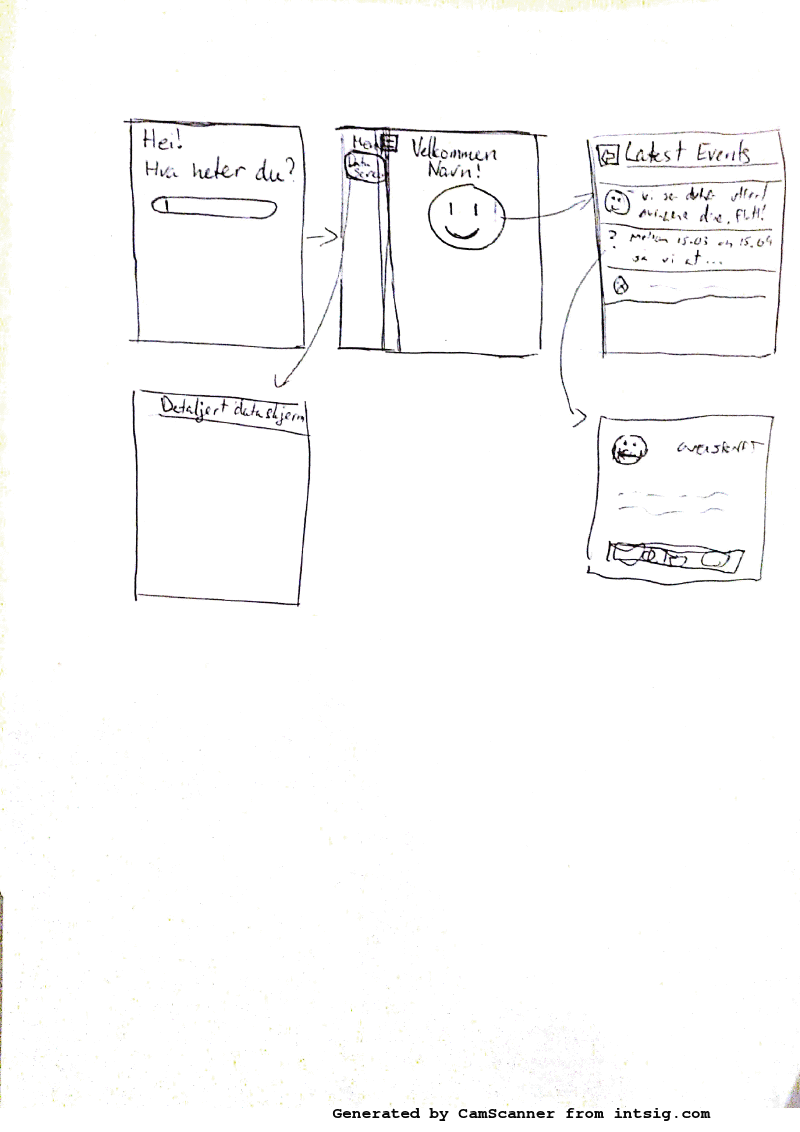
\includegraphics[trim = 20mm 180mm 0mm 20mm, clip, width=\linewidth]{Res/mockupV2}}
\caption{A mockup of the program flow, text is just scribbling}
\label{fig:mockupV2}
\end{figure}


\section{Reports}

\begin{figure}
\begin{tabular}{|c|c|p{7cm}|}
\hline
Sprint nr. & Date & Summary\\
\hline
Sprint 1: & 03.02.13 - 08.02.13 & Developing user stories and paper prototypes of the GUI.\\ 
\hline
Sprint 2: & 08.02.13 - 15.02.13 & Developing a mock-up application demonstrating the GUI.\\
\hline
Sprint 3: & 15.02.13 - 22.02.13 & Improving UI and functionality for the prototype, researching medicinal factors. \\
\hline

\end{tabular} 
\label{tab:sprintList}
\caption{Short summary of work done sorted by sprint}
\end{figure}

\end{document}
